\documentclass[a4paper]{article}
\usepackage{amsmath} % using math package
\usepackage{amssymb}
\usepackage{cite}
\usepackage{xcolor}
\usepackage{graphicx}

%define new command
\newcommand{\pd}{\partial}


\newcommand{\ket}[1]{\big|  #1 \big \rangle }
\newcommand{\bra}[1]{ \big\langle #1 \big | }

\newcommand {\avg}[3] {\langle {#1} |{ #2} |{#3} \rangle} 

\begin{document}

\title{The Explanation and Extension of the Stern-Gerlach Experiment}
\author{Gong Maoyan}
\date{16 Oct, 2018}
\maketitle



\begin{abstract}
In the Stern-Gerlach experiment, the existence of spin of electrons is demonstrated through analysing the results accroding to the theory of quantum measurement.
\textcolor{red}{[From an abstract, readers expect at least the summary of the article. What I learnt from the abstract above is that "the existence of spin angular momentum of electrons is illustrated by the analysis." But are you really illustrated the existence? ]}
\end{abstract}

\section{Introduction}
\quad In the year of 1922, in order to improve the theory of Space quantization which was proposed by Bohr, Otto Stern, with Walter Gerlach, did the experiment called the Stern-Gerlach Experiment. But it reveals that the electrons themselves have magnetic moments. It shows that the spin angular momentum quantum number is a half. Before the discovery of electron spin angular momentum, it has been known that orbital angular momentum quantum numbers are integers. So they opened a new era.

\section{Methods}

\begin{figure}[htbp!] \label{Appliances}
\centering % put the fig. in the center
    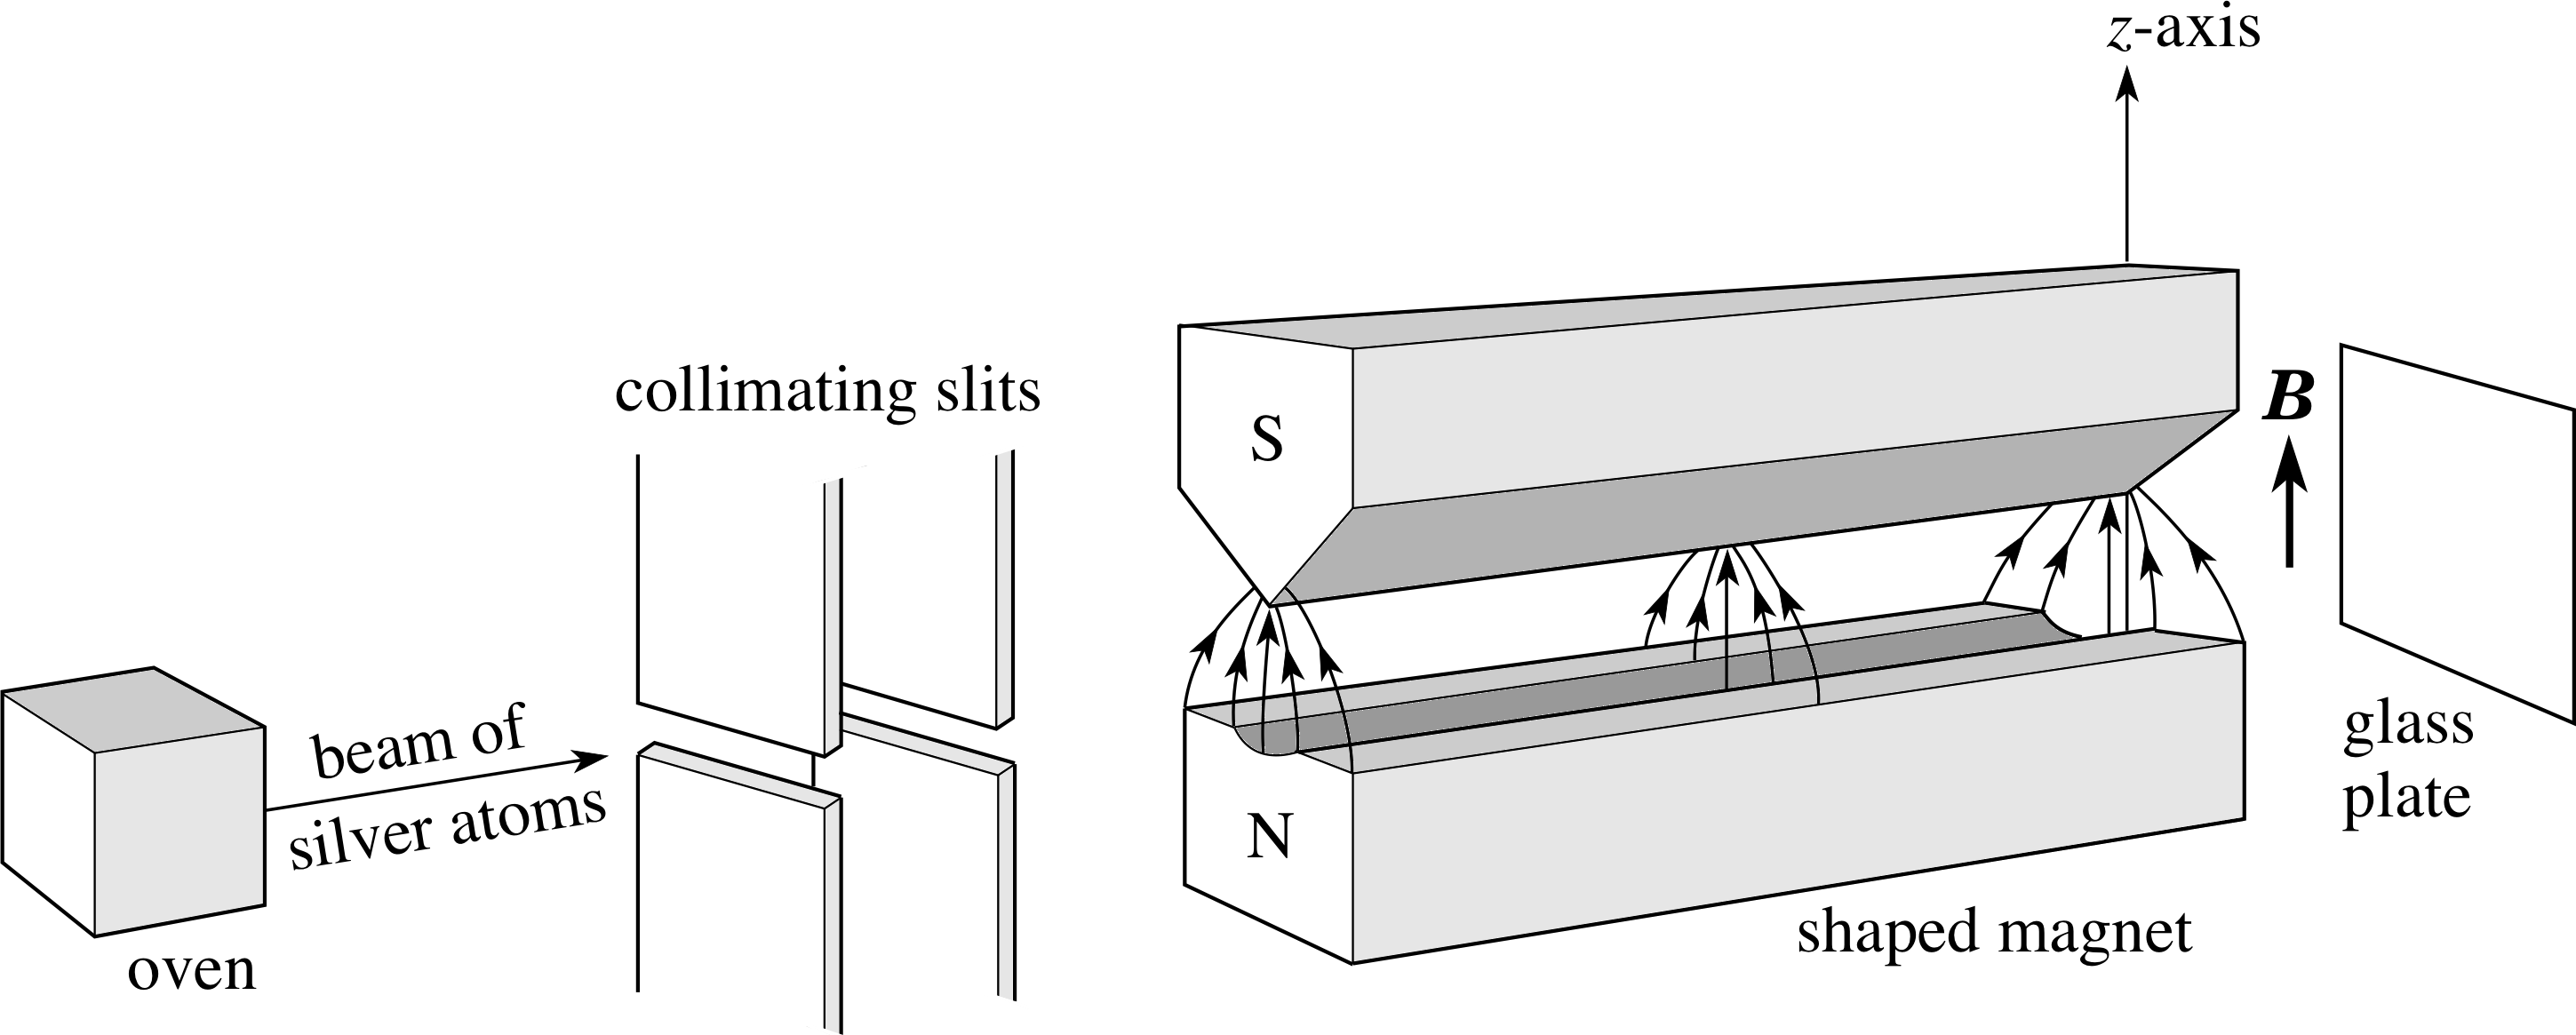
\includegraphics[width=1.0\linewidth]{Appliances.png}
    \caption{The Appliances of the Stern-Gerlach Experiment}
\end{figure}

In a vacuum chamber, silver is placed in a heating vessel, and the evaporated silver atoms are ejected from the small holes of the vessel, passing through a vertical magnetic field, and then onto the screen in the vacuum chamber, where the silver atoms condense to form traces. The result of the experiment is the Figure 2.

\begin{figure}[htbp!] \label{1st result}
\centering % put the fig. in the center
    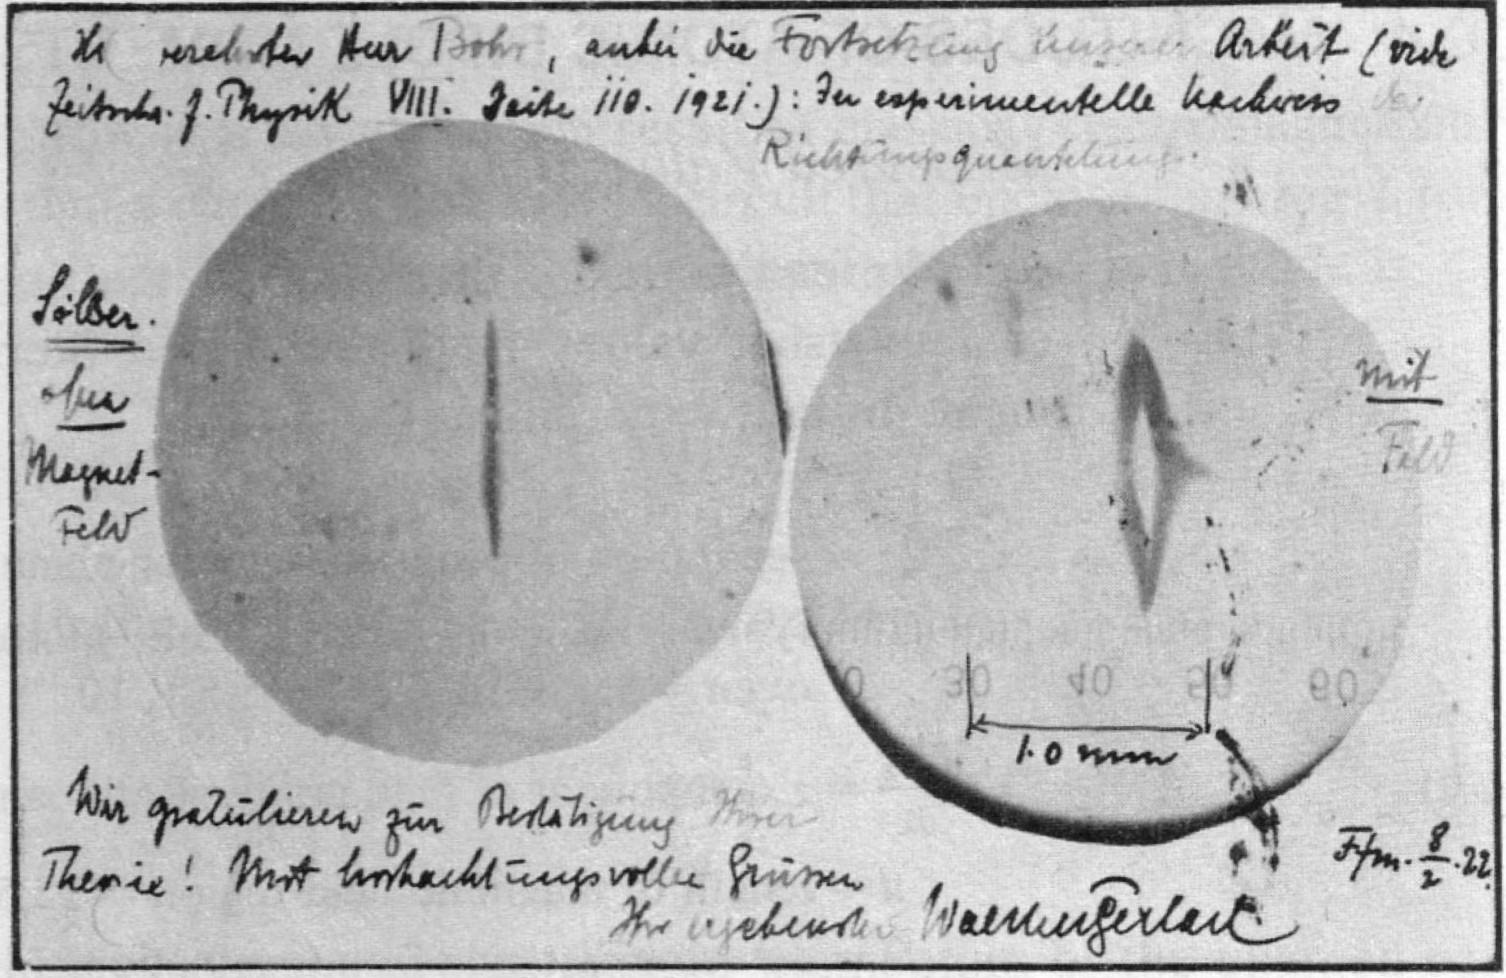
\includegraphics[width=0.8\linewidth]{1st.jpg}
    \caption{The Result 1 of the Stern-Gerlach Experiment}
\end{figure}

The Figure 2 is the postcard which Stern sent to Bohr. In the classical physics theory, since the orientation of orbital angular momentum is considered to be random, the observed trace should be a continuous distribution. But there are two symmetrical traces perpendicular to the direction of the atom flow in the picture, but there are no traces in the position of the atom flow incidence. Therefore, the Stern-Gerlach experiment confirmed the theory of spatial quantization.
\cite{FeynmanR.P.Leighton2005}

The key to the experiment is the "non-uniform magnetic field," Stern and Gallagher made special magnets with special shapes, so that the magnetic field is basically in the Z direction, and along the Z direction is non-uniform. If we carry on the continuous Stern-Gerlach experiment, it means that we put several groups of appliances, which have magnetic field in different directions together and let the silver atoms pass through the appliances one by one. What types of traces will we get on the screen? After many times of experiment, we can found the result is like the Figure 3.

\begin{figure}[htbp!] \label{2nd result}
\centering % put the fig. in the center
    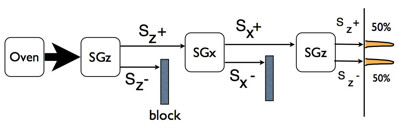
\includegraphics[width=0.8\linewidth]{2nd.jpg}
    \caption{The Result 2 of the Stern-Gerlach Experiment}
\end{figure}

\section{Results}
\quad We define the spin operator as $s=\frac{\hbar \sigma}{2}$,
$\sigma$ is a dimensionless operator. Its projection in any direction can only be $\pm1$. So
\begin{equation}
\sigma_x^2=\sigma_y^2=\sigma_z^2=1
\end{equation}
According to commutation relation
\begin{equation}
\textbf{L}\times\textbf{L}=i\hbar\textbf{L}
\end{equation}
We can get the commutation relationship of $\sigma$
\begin{equation}
\begin{cases}
\sigma_x\sigma_y-\sigma_y\sigma_x=2i\sigma_z\\
\sigma_y\sigma_z-\sigma_z\sigma_y=2i\sigma_x\\
\sigma_z\sigma_x-\sigma_x\sigma_z=2i\sigma_y
\end{cases}
\end{equation}
By calculation, you can get the equation written below.
\begin{equation}
\begin{cases}
\sigma_x\sigma_y=-\sigma_y\sigma_x=i\sigma_z\\
\sigma_y\sigma_z=-\sigma_z\sigma_y=i\sigma_x\\
\sigma_z\sigma_x=-\sigma_x\sigma_z=i\sigma_y
\end{cases}
\end{equation}
In the Stern-Gerlach experiment device, the silver atom comes out of the magnetic field in the direction of Z. Then they split into two bundles which the directions are $\ket{+}_z$ and $\ket{-}_z$. The two states correspond to $\sigma$=$\pm1$, two eigenstates. This can also be expressed as $\sigma_z$ $\ket{\pm}_z$ =$\pm  \ket{\pm}_z$.\\
The eigenstate of $\sigma_z$ can be defined from the following calculation.
\begin{equation}
\begin{pmatrix}
1&0\\0&-1\\
\end{pmatrix}
\begin{pmatrix}
a\\b\\
\end{pmatrix}
=\lambda
\begin{pmatrix}
a\\b\\
\end{pmatrix}
\Rightarrow
\begin{pmatrix}
1-\lambda&0\\0&-1-\lambda\\
\end{pmatrix}
\begin{pmatrix}
a\\b\\
\end{pmatrix}
=0
\end{equation}
So the eigenstate is $\begin{pmatrix} 1\\0\\\end{pmatrix} $ when $\lambda$ =1, the same reason, the eigenstate is $\begin{pmatrix} 0\\1\\\end{pmatrix} $ when $\lambda$ =-1.
And then, we can know,\\
$\ket{+}_z$= $\begin{pmatrix} 1\\0\\\end{pmatrix}$ $\equiv$ \ket{0}\\ $\ket{-}_z$= $\begin{pmatrix} 0\\1\\\end{pmatrix}$ $\equiv$ \ket{1}.\\
After transformation, we can get Pauli matrix under the representation of \ket{0} and \ket{1}.
\begin{equation}
\sigma_x=\begin{pmatrix} 0&1\\1&0\\\end{pmatrix},
\sigma_y=\begin{pmatrix} 0&-i\\i&0\\\end{pmatrix},
\sigma_z=\begin{pmatrix} 1&0\\0&-1\\\end{pmatrix}
\end{equation}
\quad In this experiment, the experimental device along the Z-direction acts as an optical polarization detector, indicating that the measurement will affect the state of the system, because of the interference of the experimental instrument, the measurement results will change. The calculated results show that if the second baffle is not placed in the X-direction experimental device, the atomic beam will not occur, and the theoretical values are in agreement with the experimental values.
\cite{sakurai1967advanced}

\section{Conclusion}
\quad In the Stern-Gerlach experiment, there are two values of magnetic moments. At that time, people did not have the concept of spin. According to classical theory, the orbital angular momentum can only be taken as an integer. The solution is to introduce electron spin. Spin is a physical quantity that does not correspond to classical theory. It is usually thought of as the rotation of the electron itself, but experiments have proved that this phenomenon does not exist. If so, it is contrary to relativistic theory. There are also differences between classical physics and quantum physics.

\bibliographystyle{IEEEtran}
\bibliography{Mytex}
\end{document}

